\chapter{Appendix}
\label{a:appendix}

\section{Software Manual}
\label{s:softwaremanual}

The easiest way to play a few hands against UZHoldem is by using Poker Academy. After downloading and installing Poker Academy, the necessary files (found in uzholden-dist.zip) have to be added to the program folder of Poker Academy.


\begin{figure}[!h]\centering
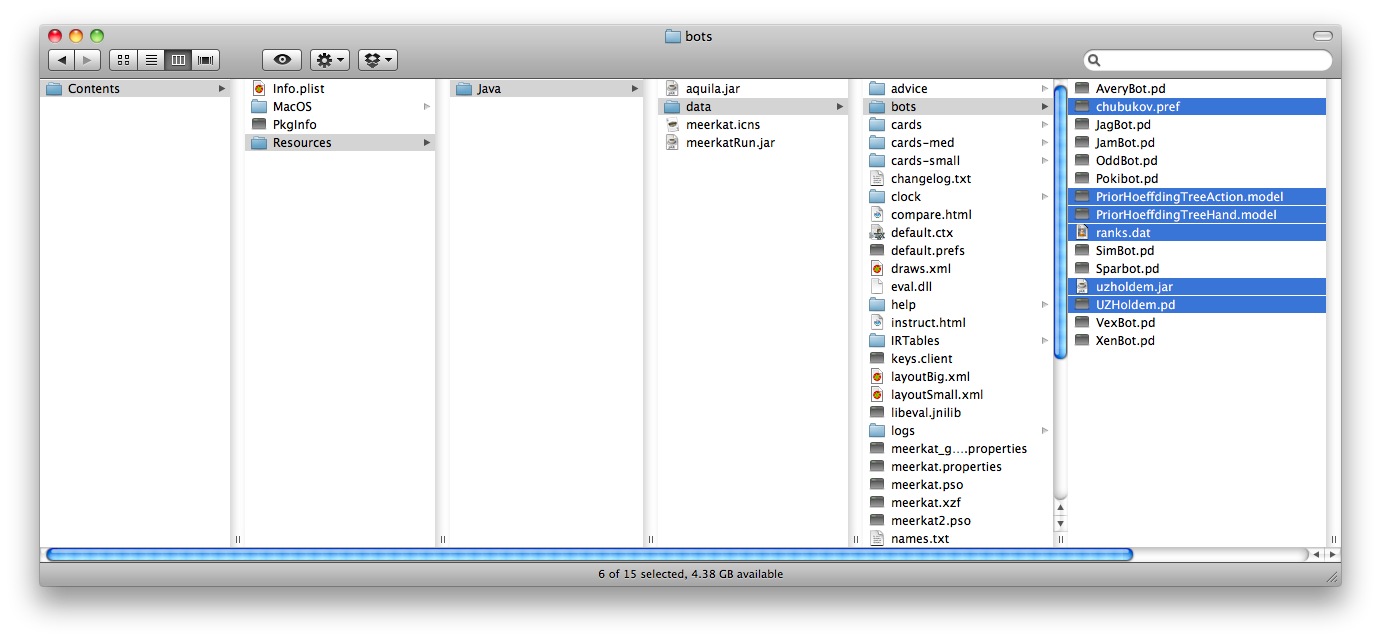
\includegraphics[width=0.65\linewidth]{section-appendix/figures/file-location}
\caption{Target location of the required files}
\label{fig:file-location}
\end{figure}
\begin{figure}[!ht]\centering

\subfigure[The opponent manager is found in the "Window" Menu ]{
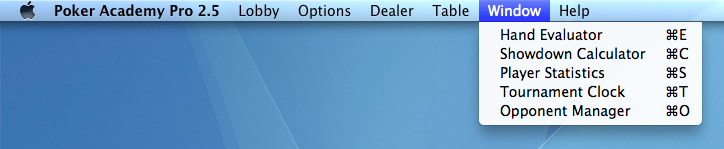
\includegraphics[width=0.65\linewidth]{section-appendix/figures/opponent-manager1}

}
\subfigure[Adding a new player]{
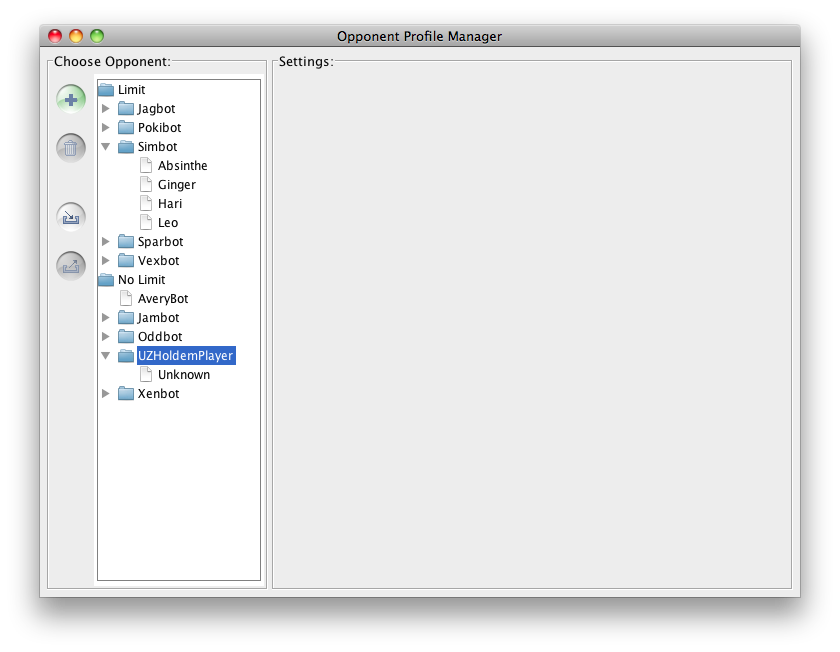
\includegraphics[width=0.65\linewidth]{section-appendix/figures/opponent-manager2}
}

\caption{Adding a new player to the opponent manager}
\label{fig:opponent-manager}
\end{figure}

Figure \ref{fig:file-location}�shows the required location of the files in the application package in Mac OS X. On Windows, the steps are similar, when copying all the files into the \texttt{data/bots}� directory.

Although its possible to use UZHoldem with the standard settings, I recommend starting PokerAcademy with a JVM that has 512MB or even 1GB memory available. On Windows, this can by done by starting Poker Academy with the switch \texttt{-JXmx512}, on Mac OSX, this requires changing the \texttt{Info.plist} file in the application package (key \texttt{VMOptions}).

 After copying the files, the only additional step required is adding a new player based on the agent (figure \ref{fig:opponent-manager})

\begin{figure}[!h]\centering
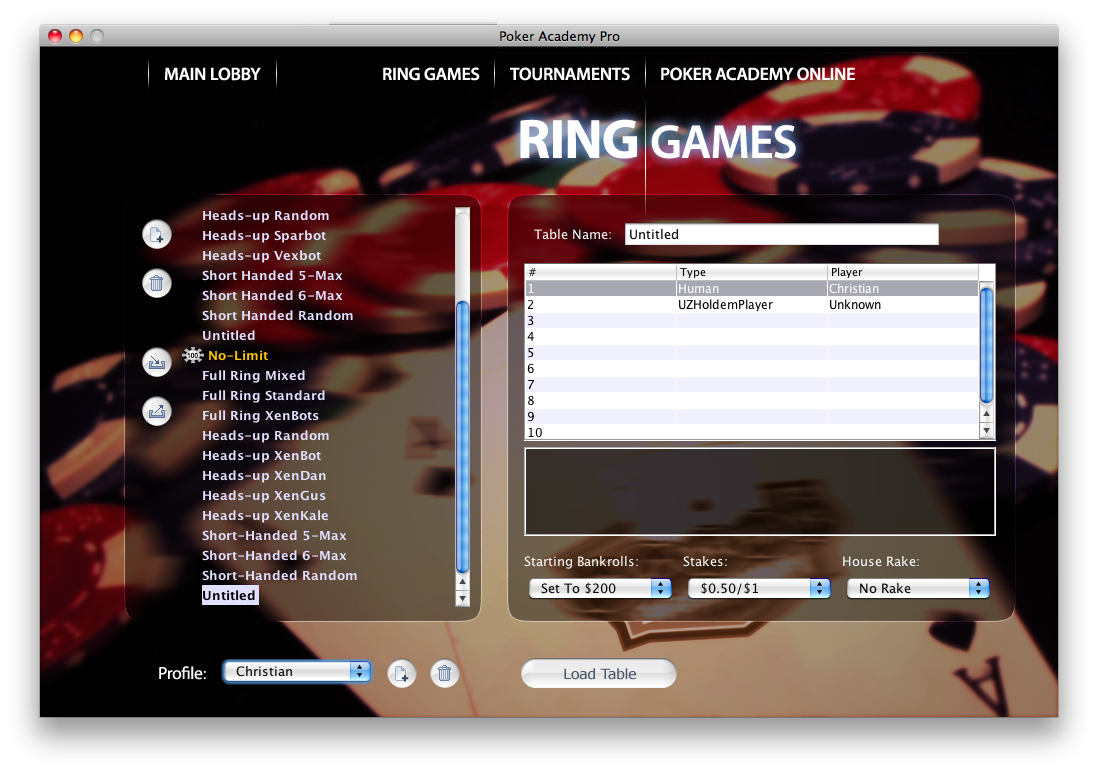
\includegraphics[width=\linewidth]{section-appendix/figures/new-table}
\caption{Creating a new table with two players}
\label{fig:new-ptable}
\end{figure}

As a final step, the opponent can now be placed on a new poker table. 
